\chapter{iBeacon} \label{chap:ibeacons}
\citet{apple:wwdc_2013_bruins} introduced at Apple's yearly \ac{WWDC} in 2013 a new technology, called \emph{iBeacon}, to enhance smartphone applications's location awareness.

An iBeacon, in general a beacon\footnote{\emph{iBeacon} is a registered trade mark of Apple}, is a System-on-Chip which emits a \emph{\acl{BLE}} signal in a predefined time interval, analogous to a lighthouse. Devices with capable hardware and software, for example iPhone since iPhone 4S and Android since version 4.3, can receive the signals, to provide the user location based services. Typically, a beacon's size is less the size of a child's hand, and is being powered with a small battery, to be independent of its environment. Thus, it easily can be attached to another object to establish a region around the object. A listening smartphone app can than notify the user when he enters or leafs a region, by estimating the proximity to the beacon \citep{apple:getting_started,binside:ds}. According to \citet{binside:ds}, typical use-cases are:
\begin{itemize}
  \item Location based marketing (e.g.\ digital coupons, digital signage of articles)
  \item Proximity sensing to an object
  \item Indoor localization and navigation (e.g.\ digital museums guide, airport guide)
\end{itemize}

After providing a brief idea what a beacon actually is, we are going to focus in the next sections on the beacons itself and the communication technology which is being used by a beacon to send its signal. Afterwards, we describe the \acs{API} provided by Apples mobile operating system iOS~8.1 to receive these signals. After forming the foundation, we present our evaluation's result, of the received signals on an iPhone 5S, which is very important for the algorithm's implementation, described in chapter~\ref{chap:pf}.


\section{Bluetooth Low Energy}\label{sec:ble}
\ac{BT} is a wireless short range communication technology with the intend to replace, resp.\ reduce the amount of, necessary cables. The technologies key features are robustness, low cost and low power consumption. It is often being used to connect a car's speaker phone with a smartphone, to connect a wireless keyboard or mouse with a computer, or to exchange files between two cell- or smartphones. The \acl{BT} standard is being developed by the \emph{Bluetooth Special Interest Group (Bluetooth SIG)}, which is a large group of companies, that are interested in \acs{BT}.

Originally, the \ac{BT} specification contained just one wireless technology system called \emph{\ac{BR}/\ac{EDR}}. Since version 4.0, released in 2010, the specification adds a second technology named \emph{\ac{LE}}. Actually, the term \ac{LE} is just the technology's name inside of the specification, but today it is also being used by the mainstream. The technologies official (marketing) label is \emph{Bluetooth Smart}. Devices labeled with it are just equipped with the \ac{LE} technology. Against, devices labeled with \emph{Bluetooth Smart Ready} are equipped with both technologies, the traditional \ac{BR} and the \ac{LE} technology \citep{bluetooth:spec}. One of the differences is the speed. \ac{BR}/\ac{EDR} has a max.\ transfer rate of 2-3~Mbps; whereas, \ac{LE} is just designed for 1~Mbps. But, \ac{LE} has the advantage of having a low current consumption. Its complexity is also lower than the one of \ac{BR}/\ac{EDR} \citep{bluetooth:spec}.

iBeacons usually are Bluetooth Smart, not Bluetooth Smart Ready devices \citep{binside:ds}. To get a better idea of how the communication between a smartphone and an iBeacon works, we give an overview of the \acs{BT} technology with focus on \acs{BLE}. Both \ac{BT} systems are using the 2.4~GHz frequency band.


\subsection*{Channels and Events}
\ac{BLE} divides the band into 40 channels. Three of them are advertisement channels, the others are data channels. These channels are being used to send events, which consists of typical (data) packets that are being send over the channels. The \ac{BLE} specification distinguishes between two event types, the \emph{advertisement} and the \emph{connection} event.

Advertisement events are either being used for unidirectional or broadcast communication, between two or more devices, or to establish a pair-wise or bidirectional communication. This type of advertisement event is called a \emph{connectable advertisement}. Advertisement events are being send via one of the advertisement channels. The device which sends the advertisement is called the \emph{advertiser}. The device looking for these events is named \emph{scanner}.

If a device listens for a connectable advertisement, it is called the \emph{initiator}, and becomes the \emph{master}, after establishing the connection. The advertising device becomes the \emph{slave}. Master and slave(s) are forming a piconet. Slaves in a piconet cannot communicate with each other. The connection establishment takes place on one of the advertisement channels. After establishing a connection, the communication takes place on the data channels by using frequency hopping instead of one specific channel \citep{bluetooth:spec}.

\subsection*{Operations}
According to \citet{bluetooth:spec}, \ac{BLE} implements different operations for the above mentioned event behavior:
\begin{itemize}
  \item To send advertisement events the \emph{Advertisement Procedure} is being used. It sends unidirectional broadcast messages, without being connected to the devices. If the device itself is already connected to another device, it can just send non-connectable advertisements. Advertisements can contain user data. A scanner can respond to a advertisement to request more user data.
  \item The \emph{Scanning Procedure} must be used to listen for advertisement packets. It can read the user data, send in an advertisement. Scanning is possible while being connected to a device.
  \item It is possible to listen just for a specific set of devices. Therefor, the \emph{Device Filtering Procedure} needs to be used.
  \item The \emph{Discovering Procedure} can be used to especially look for devices; therefor, it  uses device filtering.
  \item To establish a connection the \emph{Connecting Procedure} must be used.
  \item After the connection establishment the \emph{Connected Procedure} is used to transfer data.
\end{itemize}

\subsection*{Security}
As mentioned by \citet{bluetooth:spec}, the data is being encrypted with the \emph{AES-CCM} encryption method. For authentication, it provides three different modes for different device capabilities:
\begin{itemize}
  \item \emph{Just Works}: Requires just a possibility to tell the device, that it should accept a connection request of an unknown device. Therefor, a hardware button can be used, that the user needs to press for a few seconds, for the initial connection establishment. This is often the case to connect wireless smartphone headsets. The method is often being used, if the slave has no possibility to enter a key.
  \item \emph{Passkey Entry}: Requires the input of a PIN code. Therefor, the master needs the possibility to show a PIN code, e.g.\ on screen, and the slave needs some sort of keyboard. A typical example is the pairing process of a \ac{BT} keyboard with a computer. The computer displays a code and the user has to enter it on the keyboard that wants to connect.
  \item \emph{Out of Band}: Requires a separate channel which is being used for the discovery and also for the exchange of the secure key; for instance, a wired connection.
\end{itemize}


\subsection*{Adverting and Response Data}
Besides the mentioned user data the advertisement and response always contains data such as the \emph{local name} of the device, which can be used to identify it, information about the \emph{manufacturer}, and the \emph{Tx-power level}, which was being used to send the packets. Furthermore, it includes \emph{flags} which provide information whether the device is in limited discoverable mode, if the device supports also \ac{BR}/\ac{EDR}, if both modes can be used simultaneously, and further service specific data.


\subsection*{Summary}
\acl{LE} is a separate wireless communication technology which was added to the traditional \acl{BT} system. Devices equipped with a \ac{BT} chip of version~4, can either support both systems or just one. \ac{BLE} is low cost and has low power consumption. Thus, it is possible to produce cheap devices like iBeacons which can be powered over months with just a coin cell.

Often, the question comes up, whether beacons can be used to track users, resp.\ their smartphones. Therefor, a response from the smartphone must be send. As we have seen, advertisements do not require a response; thus, tracking would just be possible by establishing, or at least trying to establish, a connection. But due to the fact, that just one connection at the same time can be established, and thus, a device could just talk to one beacon, connection establishment cannot take place. Now we know, that the claim, made by \citet{apple:getting_started}, that tracking or putting ``user's private data at risk'' is not possible, is true.

\section{Beacon}\label{sec:beacon}
As mentioned before beacons are small System-on-Chip devices, which send \acs{BLE} signals. To manufacture beacons, compatible with Apple's iBeacon standard, or to get an insight in the official specification a license from Apple needs be obtained. Thus, we are focusing on the publicly available documentation, which describes all the interesting parts with enough detail for the purpose of this project.

In this section we are first giving an insight in the generally valid details. Afterwards, we focus on the possible configuration parameters of the beacons hardware, we use. Finally, we describe the necessary steps, after deploying the beacons.

\subsection{General Details}
In general, each beacon sends a \acs{BLE} signal in a fixed time interval. On one side, the signal contains information to uniquely identify a beacon, and on the other side, data to be able to estimate the proximity, i.e.\ the distance, between the beacon and the device itself.

\subsubsection*{Identifier}
The unique identifier consists of three parts, the \texttt{proximityUUID}, \texttt{major}, and \texttt{minor}, which together form a unique identifier. Usually, a smartphones application is not being interested in all beacons that are around, but rather in a specific subset. Thus, the application has to tell the \ac{OS} in which it is interested in. The intention of the identifier's three parts is, to build a hierarchical identifier system for beacons, to be able to range just for a subset. The following example explains the three parts and their purposes:

Imagine a grocery store's application which needs to support several branches. Each branch has multiple beacons deployed. Thus, the application is just interested in beacons belonging to the store. It also needs to know in which branch the user is being located, resp.\ in front of which beacon.

\begin{itemize}
  \item \textbf{\texttt{proximityUUID}} (16 bytes): All beacons that are belonging to the store getting the same \acl{UUID}. Thus, the application can just range for this part of the identifier, for being notified, if the \ac{OS} receives any beacon, belonging to the store.
  \item \textbf{\texttt{major}} (2 bytes): All beacons that are deployed in the same branch do have the same \texttt{major} identifier. Consequently, the app is able to differentiate between branches.
  \item \textbf{\texttt{minor}} (2 bytes): Each beacon in a branch gets a different \texttt{minor} identifier. Hence, by combining all three identifiers, the app can determine in front of which beacon in a certain branch the user is located.
\end{itemize}

By building such an hierarchy, an application can also just range for beacons of a specific branch without having a lot of overhead \citep{apple:getting_started,binside:ds}. Typically, these three parts can either be configured on the beacon itself, if not they need to be manufactured with the desired identifiers.

\subsubsection*{Proximity estimation}
As mentioned in chapter~\ref{chap:fundamentals}, there are several physical methods to estimate the distance between a sender of an radio frequency signal and the receiver. In this case the \acl{RSS} is used to estimate the proximity. Therefor, the receiver needs to know which Tx-power level was used to send the radio frequency signal. As mentioned in section~\ref{sec:ble}, \ac{BLE}, uses the 2.4~GHz frequency. According to \citet{apple:getting_started} and \citet{binside:ds}, signals in this frequency band are heavily attenuated in obstructed environments and especially by water. Consequently, the knowledge of the sender's Tx-power level is not sufficient enough to estimate the distance. Thus, a calibration value, which is the \acl{RSS} in a distance of 1~meter, is also being send to the receiver. Therefore, the below described calibration step, after deploying the beacons is necessary.

\subsection{Hardware Specification} To test and evaluate our implementation we bought ten beacons from a company called \emph{BEACONinside GmbH} from Berlin, Germany. Our beacons have the Model No.: B0001-A (HW: Rev 1.1, SW: 1.0). Figure~\ref{fig:bi:beacons} shows a 3D slice of the beacons. According to \citet{binside:ds}, the beacon's signal have a range from 0 up to 40 meters. The chipset they used is manufactured by Texas Instruments (Model CC2541). The company obtained a license from Apple to manufacture the beacons, which are compatible to Apple's iBeacon specification~\citep{binside:ds}.

\begin{figure}
	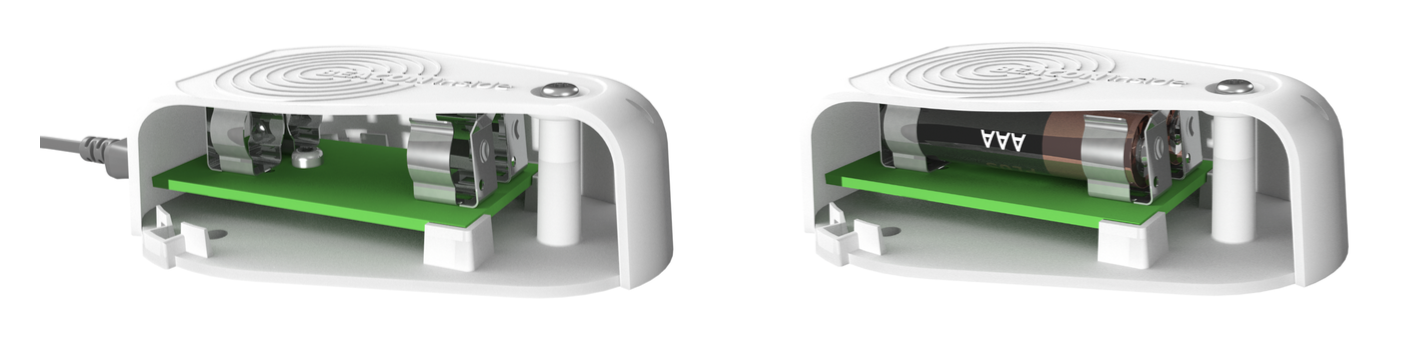
\includegraphics[width=0.6\textwidth]{figures/BEACONinside_beacons}
	\caption{Shows a 3D slice of our beacons. Source:~\citep{binside:ds}}
	\label{fig:bi:beacons}
\end{figure}

The beacons's size is $5.8~\text{cm} \times 7,96~\text{cm} \times 2.25~\text{cm}$. They can either be powered, with two AAA~batteries to provide a lifespan of approx.\ one year, or with an external power supply over micro usb~\citep{binside:ds}.

The beacons are configurable with standard \ac{BLE} tools, like capable smartphone apps. Such an app establishes a \ac{BLE} connection to the beacon. Each of the following configurable values can be accessed with a specific key. To configure the beacons we used an iOS app called \emph{LightBlue --- Bluetooth Low Energy}\footnote{Link to the LightBlue App in the iOS AppStore (last access: 18.02.2015) \url{https://itunes.apple.com/de/app/lightblue-bluetooth-low-energy/id557428110}} from a company named \emph{Punch Through Design LLC.}, recommended by BEACONinside. According to \citet{binside:ds}, the following values are configurable:
\begin{itemize}
  \item \textbf{\texttt{proximityUUID}:} For instance \texttt{F0018B9B-7509-4C31-A905-1A27D39C003C}
  \item \textbf{\texttt{major}:} A value between 1 -- 65535
  \item \textbf{\texttt{minor}:} A value between 1 -- 65535
  \item \textbf{\texttt{Tx-power level}:} It defines the power which is being used to send the beacons advertisement packets, resp.\ the signals. It can either be 0~dBm (default) which is the maximum power, -6~dBm or -23~dBm which is the minimum power level.
  \item \textbf{\texttt{Advertising interval}:} Defines the time interval (100~ms -- 10~s) in which advertisements are being send. The default time interval is 400~ms, configurable in steps of 625~$\mu$s.
  \item \textbf{\texttt{Calibration value}:} To estimate the distance of the receiving device to the beacon, a calibration step is necessary. The measured \acs{RSS} in a distance of one~meter, needs to be send by the beacon, with every advertisement. This value can be configured for each \texttt{Tx-power level}. The default is 65~dBm for the 0~dBm power level. It needs to be encoded as the 2' complement in hexadecimal (e.g.\ $65~\text{dBm} = \text{0xBF}$).
  \item \textbf{\texttt{Passkey}:} To write a property the (6 decimal digit) passkey must be entered. The beacons's default value is \texttt{555555}.
\end{itemize}

 Additionally, the following read-only properties about the device, and its state are being provided~\citep{binside:ds}:
\begin{itemize}
  \item \textbf{\texttt{Device Name}:} The beacon's name consisting of \texttt{BEACON} and the latter three bytes of its \acs{MAC} address.
  \item \textbf{\texttt{Model Number}}
  \item \textbf{\texttt{Serial Number}}
  \item \textbf{\texttt{Hardware Revision Number}}
  \item \textbf{\texttt{Software Revision Number}}
  \item \textbf{\texttt{Manufacturer Name}}
  \item \textbf{\texttt{Battery Level}:} In percent.
  \item \textbf{\texttt{Temperature}:} The hardware's temperature in degrees Celsius.
\end{itemize}

To load the new values after changing the beacon's configuration, the beacon needs to be rebooted by setting a specific value. The beacon can also be reset to factory defaults~\citep{binside:ds}.

\subsection{Deployment and Calibration}
As mentioned before, the \ac{BLE} signals quality is heavily influenced by physical materials due to the fact that \ac{BLE} uses the 2.4~GHz frequency. Especially, water which is a main part of the human body, attenuates the signal~\citep{apple:getting_started}. Thus, the beacons need to be carefully deployed in its environment. Ideally, they should be deployed in a manner, that most often the line between beacon and receiver is unobstructed. There should also be enough space around the beacon, that its signal can spread out. By deploying them carefully, the signal's attenuation, and other effects like multi-path fading and shadowing can be reduced~\citep{apple:getting_started,IEEE:survey_wireless_indoor_pos}.

The next step is the calibration step. To be able to estimate the distance between smartphone and beacon a reference value is needed. The reference value as mentioned before, is the measured \ac{RSS} in a distance of 1~m to the beacon. The calibration value is being configured on the beacon itself, which includes it in the send advertisement, together with its identifier.

According to \citet{apple:getting_started}, the smartphone needs to be positioned in 1~m distance to the beacon in portrait mode, with the device's top half uncovered. Than the \ac{RSSI} values where collected for at least 10~seconds. Meanwhile, the user should slowly move the device on an approx.\ 30~cm line in front of the beacon, by maintaining distance and orientation. After collecting the values, the average value is being calculated and configured on the beacon. It is advisable, to double check the device's estimated distance, after setting the calibration value. Due to the above mentioned problems, this needs to be repeated for every single beacon.

\section{API --- iOS 8.1}
After imparting, what beacons are and how they work, we now focus on the receivers side, especially on the \acs{API} provided by Apple's iOS~8.1 platform. The \ac{CL} framework, provides in terms of iBeacons two functionalities, called \emph{region monitoring} and \emph{beacon ranging} \citep{apple:ios_doc_cl}.

\subsection*{Region monitoring}
As the name already implies, the operating system monitors a specified region and notifies the application, when the user did enter or left the region. This functionality is not restricted to regions that are marked by beacons. It already existed long before, and monitors also circular regions specified, by a distance around a global position in longitude and latitude.
iOS monitors the specified regions also if the application is in background mode or is currently not running. If the user enters or leaves a region, the application is being started; for instance, to notify the user \citep{apple:wwdc_2012_bruins,apple:wwdc_2013_bruins,apple:ios_doc_cl}.

\subsection*{Proximity to a Beacon}
To continuously estimate the proximity to a beacon, ranging must be used. Therefor, a \texttt{CLBeaconRegion} needs to be specified. The \texttt{CLBeaconRegion} object requires at least the beacon's \texttt{proximityUUID}. It is also possible to specify a more specific beacon group, by adding the groups \texttt{major} identifier. By additionally passing a \texttt{minor} identifier, the framework just ranges for one specific beacon~\citep{apple:wwdc_2013_bruins,apple:ios_doc_cl}.

After starting the ranging, the framework starts to notify the before specified \texttt{delegate} in a continuously manner, after it received the first advertisement of a beacon, which it is supposed to range for. This means that, the framework does not call the \texttt{delegate}, until it receives the first matching beacon advertisement. After the first call it continuously calls the delegate approximately every second, regardless of whether it actually received a beacon's advertisement or not.

The delegate gets passed an array of \texttt{CLBeacon} objects. Each of it, represents one beacon. Table~\ref{tab:beaconExampleData} shows two example data sets, which the \texttt{CLLocationManager} passes to its delegate. Each data set contains four \texttt{CLBeacon} objects. The table's last entry represents a beacon, which is out of range.

\begin{table}
	\begin{tabular}{*{7}{c}}
time & proximityUUID & major & minor & proximity & accuracy & rssi \\
\hline
1.0400 & F0018B9B-\dots-1A27D39C003C & 21500 & 48945 & 2 & 1.2915 & -67\\
1.0400 & F0018B9B-\dots-1A27D39C003C & 39821 & 56686 & 2 & 5.9948 & -79\\
1.0400 & F0018B9B-\dots-1A27D39C003C & 41738 & 1201 & 3 & 6.8129 & -80\\
1.0400 & F0018B9B-\dots-1A27D39C003C & 38722 & 6270 & 3 & 7.7426 & -81\\
 & & & & & & \\
2.0387 & F0018B9B-\dots-1A27D39C003C & 21500 & 48945 & 2 & 1.4452 & -68\\
2.0387 & F0018B9B-\dots-1A27D39C003C & 39821 & 56686 & 3 & 5.5235 & -78\\
2.0387 & F0018B9B-\dots-1A27D39C003C & 41738 & 31201 & 3 & 6.8129 & -80\\
2.0387 & F0018B9B-\dots-1A27D39C003C & 38722 & 6270 & 0 & -1 & 0\\
\end{tabular}

	\caption{Shows recorded beacon example data. Each row represents a \texttt{CLBeacon} object. The table contains two successive datasets.}
	\label{tab:beaconExampleData}
\end{table}

A \texttt{CLBeacon} object contains on one side the beacon's identifiers, as described in section~\ref{sec:beacon}. On the other side, it contains three values, which express the beacons proximity in different ways.

\paragraph{\acs{RSSI} Property} The \texttt{rssi} property stores the \acl{RSS} measured in dBm. It expresses how strong the received signal is. As mentioned before, a beacon's advertisement time interval can be specified. Remember, the beacons we use are sending their advertisement, per default, every $400$~ms. The framework itself does stick to its $\approx$~1~s time interval. It collects all received advertisements and calculates the average since the last reported \texttt{rssi} value. If a beacon's signal was received before, but not during the current time interval, its \texttt{rssi} value is 0 \citep{apple:wwdc_2013_bruins,apple:ios_doc_cl}.

\paragraph{Proximity Property} The \texttt{proximity} property's value expresses the relative distance to a beacon. It can either be \texttt{unknown = 0}, \texttt{immediate = 1}, \texttt{near = 2}, or \texttt{far = 3}. \texttt{unknown} means, that the proximity could not be detected. One reason could be, that the ranging just started, but could not collect enough advertisements. \texttt{immediate} ``represents a high level of confidence that the device is physically very close to the beacon''~\citep{apple:getting_started}. The \texttt{near} state is reported, if the user is in approx.\ 1 -- 3~m proximity to the beacon; thus, \texttt{immediate} is reported if the user is closer than $\approx$~1~m. Consequently, the value is \texttt{far} if the ``beacon device can be detected but the confidence in the accuracy is too low to determine either Near or Immediate''~\citep{apple:getting_started}; hence, the estimated distance is larger than $\approx$~3~m.

\paragraph{Accuracy Property} The object's \texttt{accuracy} property actually, expresses the proximity to a beacon in meters, but \citet{apple:ios_doc_cl} describes the property in its iOS~8.1 documentation as follows:
\begin{quote}
  ``The accuracy of the proximity value, measured in meters from the beacon.
  [\dots]
  Indicates the one sigma horizontal accuracy in meters. Use this property to differentiate between beacons with the same proximity value. Do not use it to identify a precise location for the beacon. Accuracy values may fluctuate due to RF interference.''\citep{apple:ios_doc_cl}
\end{quote}
Thus, we did first interpret this description, as the error of the \texttt{proximity} property's value, measured in meters. But, this makes of course not much sense, because the \texttt{proximity} value stores a relative value, which already implies that the user's proximity to the beacon is in a certain range.

According to \citet{wang:bt_pos}, the distance $d$, between an iBeacon and a smartphone, which depends on the \acl{RSS}, can be calculated with the formula $d = 10^{-\frac{RSSI + A}{10 * n}}$, where $A$ is the \acs{RSSI} value at a distance of $1~m$, and $n$ an environmental constant. To proof our assumption, that the \texttt{accuracy} value is actually the distance, we did some test measurements, and compared them with our own calculations. Therefor, we measured the \acs{RSSI} for certain reference distances, and stored the associated \texttt{accuracy} values. The measurements where taken outdoor with \ac{LOS} between beacon and smartphone, to have the signals quality as less impacted by physical materials as possible. After collecting 60 measurements for each reference distance, we sorted the data set according their \texttt{rssi} values, and calculated the average of the \texttt{accuracy} values per \texttt{rssi}. Afterwards, we used the above mentioned formula to calculate the distance for each measured \texttt{rssi} value.

During the measurements, the beacon's calibration value was set to 65~dBm; thus, $A = 65~\text{dBm}$. To approximate the \texttt{CLBeacon} object's \texttt{accuracy} property best, an environmental constant of $n = 2.1$ was used, which is similar to the one used by \citet{wang:bt_pos}. Figure~\ref{fig:eval_accuracy_vs_distance} illustrates the result and the fact, that the \texttt{CLBeacon} object's \texttt{accuracy} property, is the estimated distance, between beacon and smartphone. Additionally, it implicitly depicts, that the unit $dB$ is a logarithmic unit.

\begin{figure}
  \begin{tikzpicture}
    \begin{axis}[width=0.9\textwidth, height=0.45\textheight,
        xlabel={\acl{RSS} (dBm)},
        ylabel={Estimated Distance (m)},
        legend pos=north west,
        legend entries={measurement, avg.\ \texttt{accuracy} per \texttt{rssi}, $d = 10^{-\frac{RSS + 65}{10 * 2.1}}$},
      grid = major,
      x dir=reverse, ymin=0]
      \addplot [only marks, mark=x] table[col sep=semicolon, x=rssi, y=accuracy] {csv/2014-10-15_hoehenweg/all.csv};
      \addplot [red, mark=triangle*, mark size=3pt] table[col sep=semicolon, x=rssi, y=avgAccuracy] {csv/2014-10-15_hoehenweg/all_avg_accuracy_per_rssi.csv};
      \addplot[blue, domain=-55:-95, samples=100]{10^(-(x+65)/(10*2.1))};
  \end{axis}
\end{tikzpicture}

	\caption{Dependency on \texttt{CLBeacon} object's \texttt{rssi} and \texttt{accuracy} properties \citep{apple:ios_doc_cl,wang:bt_pos,kotanen:exp_local_pos_bt}.}
	\label{fig:eval_accuracy_vs_distance}
\end{figure}

% The estimated distance in meters between the beacon and the device. If beacon's signal was received before but not in this time intervall the value is -1.
% Wenn es genauigkeit wäre müsste es an den Übergängen von klein zu groß ja auch einen sichtbaren unterschied geben


\section{Evaluation}\label{sec:beacon_eval}
After explaining how beacon advertisements can be received with Apple's mobile operating system and which data can be accessed, we evaluate the data, especially the \texttt{accuracy} property's values, which is the data being used for the later discussed algorithm. First, we focus on the distance estimations's quality, in terms of its error, under different environmental circumstances. Afterwards, we present the result of our experiment, of using pure multilateration, as introduced in section~\ref{sec:fund_trilateration}, to implement a simple localization algorithm.

\subsection{Distance Estimation}
%As mentioned before, the signals are heavily influenced by physical materials, which also has an impact on the estimated distance.
%Thus, obstacles between sender and receiver are impacting the distance estimation and as well the environments construction.
%But physical materials are not the only reason.
%The device's relative attitude to the beacon

The measured distances provided by the \texttt{CLBeacon} object's \texttt{accuracy} property varies in dynamic, but also in steady and unobstructed environments.

\paragraph{Mapping} The first reason is, that the \texttt{rssi} values are not directly mapped to the \texttt{accuracy} values. Apple's \ac{CL} framework seems to apply a filter, to estimate the distance. We recorded the \texttt{CLBeacon} object's properties over time at a fixed position, with a distance of 2~m to the beacon. We directly began recording the data after positioning the phone. Figure~\ref{fig:beacon_eval_accuracy-rssi} illustrates the behavior, by showing the \texttt{rssi} values and their corresponding \texttt{accuracy} values over time. The graph shows, that the \texttt{accuracy} values slowly converge against the actual distance of 2~m. It also shows, that outliers in the \texttt{rssi} property, do not have a direct impact, on the estimated distance.

\begin{figure}
	\begin{tikzpicture}
    \begin{axis}[width=0.9\textwidth, height=0.45\textheight,
      xlabel={Time (sec)},
      axis y line*=left,
      ylabel={Estimated Distance (m)},
        legend pos=south west,
      legend entries={\texttt{accuracy}, ref.\ distance}]
      \addplot [blue, mark=x] table[col sep=semicolon, x=time, y=accuracy] {csv/2014-10-27_htwg_f007/04_2m.csv};
      \addplot [black, dashed, domain=0:54, samples=2]{2};\label{distance}
  \end{axis}
  \pgfplotsset{every axis y label/.append style={rotate=180, yshift=15cm}}
  \begin{axis}[width=0.9\textwidth, height=0.45\textheight,
    axis y line*=right,
    ylabel={\acl{RSS} (dBm)},
    hide x axis,
    y dir=reverse,
    legend entries={\texttt{rssi}}]
    \addplot [red, mark=*] table[col sep=semicolon, x=time, y=rssi] {csv/2014-10-27_htwg_f007/04_2m.csv};
  \end{axis}
\end{tikzpicture}

	\caption {Dependency of the \texttt{CLBeacon} object's \texttt{accuracy} and \texttt{rssi} property over time with an actual distance of $2m$.}
	\label{fig:beacon_eval_accuracy-rssi}
\end{figure}

\paragraph{Attitude \& Obstacles} The second reason is the device's attitude, relative to the beacon. Figure~\ref{fig:beacon_eval_situations} shows the impact on the estimated distance and the \acs{RSS} in typical situations.
For each situation the actual distance between the two devices was 1~m. The measurements where taken indoor. The values shown in figure~\ref{fig:beacon_eval_situations} are average values. For each situation, 60 -- 100 values where recorded.\newline

\textbf{Situations:}
\begin{itemize}
  \item \emph{(1)} Horizontal iPhone in front of vertical beacon with \acs{LOS}.
  \item \emph{(2)} Horizontal iPhone sideways with \acs{LOS} to vertical beacon.
  \item \emph{(3)} Horizontal iPhone below vertical beacon with \acs{LOS} (Distance 1m, $45^\circ$ below beacon).
  \item \emph{(4)} Vertical iPhone in front of vertical beacon with \acs{LOS}.
  \item \emph{(5)} Horizontal iPhone in front of horizontal beacon with \acs{LOS}.
  \item \emph{(6)} Horizontal iPhone in front of vertical Beacon with person in between.
  \item \emph{(7)} Horizontal backwards turned iPhone in front of vertical Beacon with \acs{LOS}.
  \item \emph{(8)} Horizontal backwards turned iPhone in front of vertical Beacon with person in between.
  \item \emph{(9)} Horizontal iPhone in front of vertical Beacon with 30 cm ferro concrete wall in between.
\end{itemize}

Situation 1, 2, 5 and 7 shows, that if the iPhone is horizontal in front of or sideways of the vertical beacon with \acs{LOS}, the \acs{RSS} attenuation is at the least. Against, if the signals are received by the phone, with a different angle to the beacon, shown in situation 3 and 4, the attenuation increases.

Figure~\ref{fig:beacon_eval_accuracy-rssi} depicts also the third reason, which are static obstacles such as walls, or the user's own body.

A human body between the phone and a beacon, shown in situation 6 and 8, has a much higher impact. The estimated distance increases in approx.\ 3 meters. Whereas, a ferro concrete 30~cm wall, shown in situation 9, drastically impacts the distance. The phone estimates a distance of 9~meters instead of 1~meter.

The above illustrated scenarios are very common. The problem is, that it is not distinguishable, if a estimated distance is being impacted by the attitude, a wall, or a person, without knowing its own exact position, the beacons attitude, and the positions of all obstacles.\newline

\begin{figure}
	\subfloat[The average estimated distance in different situations.]{
  \begin{tikzpicture}
    \begin{axis}[width=0.45\textwidth, height=0.35\textheight,
        xlabel={Situation},
        ylabel={Estimated Distance (m)},
        xtick=data,
        legend entries={\texttt{accuracy}},
        legend pos = north west,
      grid = major]
      \addplot [only marks, mark=*] table[col sep=semicolon, x=measurement, y=accuracy] {csv/2014-10-27_htwg_fk034_angles/all_avg.csv};
  \end{axis}
\end{tikzpicture}
}
\subfloat[The average \acs{RSS} in different situations.]{
  \begin{tikzpicture}
    \begin{axis}[width=0.45\textwidth, height=0.35\textheight,
        xlabel={Situation},
        ylabel={\acl{RSS} (dBm)},
        y dir=reverse,
        xtick=data,
        legend entries={\texttt{rssi}},
        legend pos = north west,
      grid = major]
      \addplot [only marks, mark=*] table[col sep=semicolon, x=measurement, y=rssi] {csv/2014-10-27_htwg_fk034_angles/all_avg.csv};
  \end{axis}
\end{tikzpicture}
}

	\caption {Depicts the impact of the phones attitude, relative to the beacon, and obstacles, such as humans or walls, on the \acs{RSS}.} %  The measurements where taken indoor (HTWG Konstanz FK034) with an actual distance of 1~m between iBeacon and smartphone.
	\label{fig:beacon_eval_situations}
\end{figure}


\paragraph{Spreading \& Error} To depict that the estimated distance also varies in steady unobstructed environments with \acs{LOS}, we recorded the \texttt{accuracy} values, for different reference distances in different environments. Therefor, we recorded for each reference distance 60 values. We calibrated the used beacon for each environment.

Figure~\ref{fig:beacon_dispersion_outdoor} illustrates the collected \texttt{accuracy} values measured at 1, 2, \ldots, 5, 10, \ldots, 30~meters distance to the beacon. The measurements where taken outdoor with \acl{LOS} between the two devices.

The graph shows, that the average \texttt{accuracy} measured at 1 -- 4~m distance is very close to the actual distance. It also shows, that the value's spreading for these distances, is very low. For distances $\geq$~5~m, the spreading increases and sways between small and huge; thus, it is not correlated to the reference distance. 
% Compared to the measurements of 1, \ldots, 4 meters the error increases and sways.

As mentioned before the beacons manufacturer claims a maximum range of 40~m. We could range the beacon in this scenario, up to a distance of 42~m.

We repeated the exact same experiment in an indoor environment. The results are depicted in figure~\ref{fig:beacon_dispersion_f-cellar}. Also in this case the average \texttt{accuracy} comes very close to the actual distance with a very low spreading for the first 4 distances. At 5~m the spreading and error increases and sways, too.

Interestingly, the spreading starts to decreases between 10 -- 30~m, from a very large to a much smaller value. At the same time the error grows, because due to the \acs{RSS}, the smartphone estimates a very small distance; whereas, the actual distance is very large. The assumed reason is the test environment's construction form. The measurements where recorded in a straight, long, but slim, corridor in a cellar. There are multiple doors, made of steel, on both sides of the wall, that maybe caused reflections.

The depicted measurements in figure~\ref{fig:beacon_dispersion_f007} are recorded in an approx.\ 15~m long and 8 -- 11~m wide lecture hall. It shows, that also the first few meters on average are matching best, but it also depicts, that there are sometimes huge differences in the estimated distance, at the same position.

\begin{figure}
	\subfloat[Measured outdoor]{
  \begin{tikzpicture}
    \begin{axis}[trim axis left, trim axis right, width=0.45\textwidth, height=0.45\textheight,
        xlabel={Reference Distance (m)},
        ylabel={Estimated Distance (m)},
        legend pos=north west,
        legend entries={\texttt{accuracy}, avg. \texttt{accuracy}},
        grid = major]
      \addplot [only marks, mark=x] table[col sep=semicolon, x=proximityRef, y=accuracy] {csv/2014-10-15_hoehenweg/all.csv};
      \addplot [red, only marks, mark=triangle*, mark size=3pt] table[col sep=semicolon, x=proximityRef, y=avgAccuracy] {csv/2014-10-15_hoehenweg/avg_all.csv};
      \addplot [black, dashed, domain=0:30, samples=2]{x};
  \end{axis}
\end{tikzpicture}
\label{fig:beacon_dispersion_outdoor}
}
\subfloat[Measured in basement (HTWG-KN F)]{
  \begin{tikzpicture}
    \begin{axis}[width=0.45\textwidth, height=0.45\textheight,
        xlabel={Reference Distance (m)},
        ylabel={Estimated Distance (m)},
        legend pos=north west,
        legend entries={\texttt{accuracy}, avg. \texttt{accuracy}},
        grid = major]
      \addplot [only marks, mark=x] table[col sep=semicolon, x=proximityRef, y=accuracy] {csv/2014-10-15_htwg_keller_f/all.csv};
      \addplot [red, only marks, mark=triangle*, mark size=3pt] table[col sep=semicolon, x=proximityRef, y=avgAccuracy] {csv/2014-10-15_htwg_keller_f/all_avg_accuracy_per_proximity.csv};
      \addplot [black, dashed, domain=0:30, samples=2]{x};
  \end{axis}
\end{tikzpicture}
\label{fig:beacon_dispersion_f-cellar}
}

\subfloat[Measured in lecture hall (HTWG-KN F007)]{
\begin{tikzpicture}
    \begin{axis}[width=0.45\textwidth, height=0.45\textheight,
        xlabel={Reference Distance (m)},
        ylabel={Estimated Distance (m)},
        legend pos=north west,
        legend entries={accuracy, avg. accuracy},
        legend entries={\texttt{accuracy}, avg. \texttt{accuracy}},
        grid = major]
      \addplot [only marks, mark=x] table[col sep=semicolon, x=proximityRef, y=accuracy] {csv/2014-10-27_htwg_f007/all.csv};
      \addplot [red, only marks, mark=triangle*, mark size=3pt] table[col sep=semicolon, x=proximityRef, y=avgAccuracy] {csv/2014-10-27_htwg_f007/all_avg_accuracy_per_proximity.csv};
      \addplot [black, dashed, domain=0:14.5, samples=2]{x};
  \end{axis}
\end{tikzpicture}
\label{fig:beacon_dispersion_f007}
}

	\caption {Shows the \texttt{accuracy}'s spreading depending on the actual distance and the environment.}
	\label{fig:beacon_dispersion}
\end{figure}


\paragraph{Uncertainty} As mentioned in section~\ref{sec:fund_loc}, it is necessary to know the uncertainty of a measurement, to implement a particle filter. Thus, we determined distance estimations uncertainty based on the data shown in figure~\ref{fig:beacon_dispersion_outdoor} and \ref{fig:beacon_dispersion_f007}. The gaussian's parameters, to model the distance estimation's uncertainty, are depicted in figure~\ref{fig:beacon_eval_ndf}. The two dashed straight lines show the linear function that approximates the standard deviation $\sigma$ depending on the mean $\mu$ best.

\begin{figure}
	\begin{tikzpicture}
    \begin{axis}[trim axis left, trim axis right, width=0.9\textwidth, height=0.45\textheight,
        %title={Normal Distribution Function parameters},
        xlabel={Mean $\mu$ (m)},
        ylabel={Standard deviation $\sigma$ (m)},
        legend pos=south east,
        legend entries={outdoor, $f(\mu)=0.3286 \cdot \mu + 0.8379$, indoor (HTWG-KN F007), $f(\mu)=0.3131 \cdot \mu + 0.0051$},
      grid = major]
      \addplot [red, mark=*] table[col sep=semicolon, x=mu_distance, y=sigma_distance] {csv/2014-10-15_hoehenweg/ndf_parameters.csv};
      \addplot [red, dashed, domain=0:30, samples=2]{0.3286*x+0.8379};
      \addplot [blue, mark=*] table[col sep=semicolon, x=mu_distance, y=sigma_distance] {csv/2014-10-27_htwg_f007/ndf_parameters.csv};
      \addplot [blue, dashed, domain=0:30, samples=2]{0.3131*x+0.0051};
  \end{axis}
\end{tikzpicture}

	\caption{Depicts the uncertainties of the distance estimation modeled with a normal distribution function.}
	\label{fig:beacon_eval_ndf}
\end{figure}


\subsection{Multilateration}
After evaluating the distance estimation's quality of one beacon, we decided to deploy some beacons in a lecture hall to get a better feeling, of how good the distance estimation actually works. On one side, the goal was to visualize the estimated distances on a map, to proof their plausibility, and on the other side, to test if indoor self-localization with smartphones is possible by just using iBeacons, without integrating additional sensor data.

As already mentioned in section~\ref{sec:fund_trilateration}, \emph{multilateration} is a method to estimate the position, by using the distances to several senders. The receivers position by using just one sender is somewhere on a circle around the sender with the estimated distance as radius of the circle.
By using two senders $s_1$ and $s_2$, the two circles around the senders can have zero, one or two intersections, if the position of $s_1 \neq s_2$. Thus, the receivers position must be at one of the circles's intersections.
By adding a third sender $s_3$ the three circles have either no or exactly one, common intersection point, which is the receivers position. This applies also to more than three senders.

To be able to use our implementation with variable sender count, we use the \emph{Least Square} method to determine the receivers position. Another advantage is, that the least square method can also estimate a position if no common intersection point exists.

For our experiment we used the same lecture hall as before. There, we positioned four beacons. Then we used our test device, which is an iPhone~5S, to recorded the received beacon identifiers with their corresponding estimated distances, resp.\ the \texttt{accuracy} values, provided by \acs{CL}, during our test walk on a defined path.

To visualize the estimated distances to the beacons and the device's estimated position, resp.\ the walked path, we wrote a small Python program. Figure~\ref{fig:beacon_eval_multilat} shows four screenshots of the programs output. Each of it shows a map, which shows the lecture halls walls in grey. The white space in the hall, is free space. The filled small blue circles next to the walls are the four beacons. The big blue circles, are the circles around the beacons, where the radius represents the estimated distance to the beacons. We walked on the green tetragon, beginning at the bottom right corner in counter clockwise direction, with holding the test device in front of us. The beacons where positioned in approximately the same hight, as the hold device. The red line shows the path estimated.

The first screenshot, depicted in figure~\ref{fig:beacon_eval_multilat_1}, shows, that the estimated distance sometimes is completely wrong, as shown by the blue circle around the top-right beacon. It also shows that the estimated position is somewhere several meters outside of the lecture hall. The second screenshot shows, that the distance to the top-right beacon shrinks, but the one to the top-left, massively grows. The distances to the other two beacons, seem to be plausible. Figure~\ref{fig:beacon_eval_multilat_3}, shows a plausible position. It also shows, that in this step, beacon's signal, positioned at the bottom-right corner, was not received. The last screenshot shows also a more or less plausible position. The distances, except the one to the beacon, positioned at the bottom-left corner, seem to be plausible.

\begin{figure}
  \subfloat[]{
  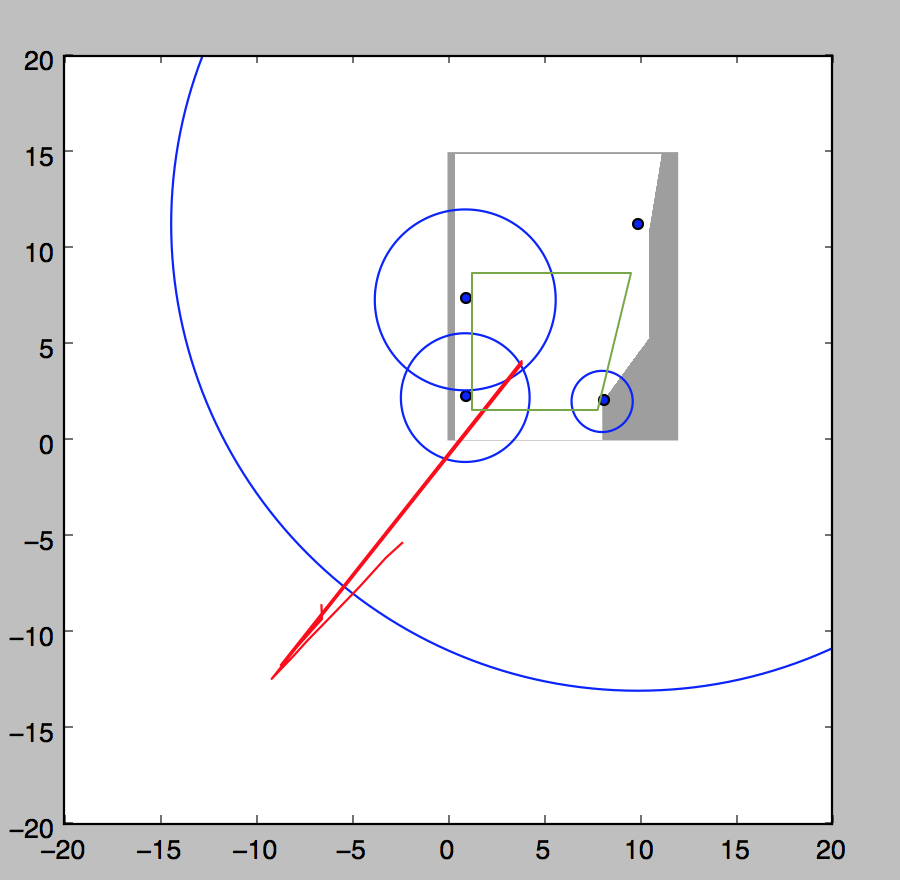
\includegraphics[width=0.45\textwidth]{figures/multilat_1}
  \label{fig:beacon_eval_multilat_1}
}
\subfloat[]{
  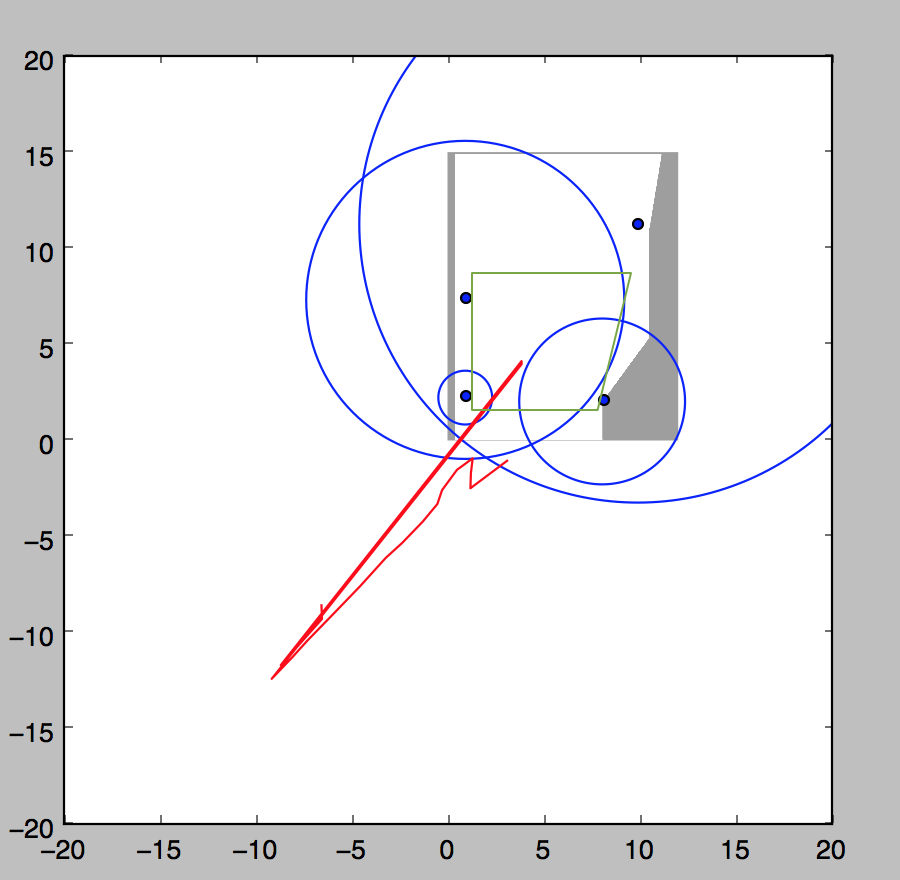
\includegraphics[width=0.45\textwidth]{figures/multilat_2}
}

\subfloat[]{
  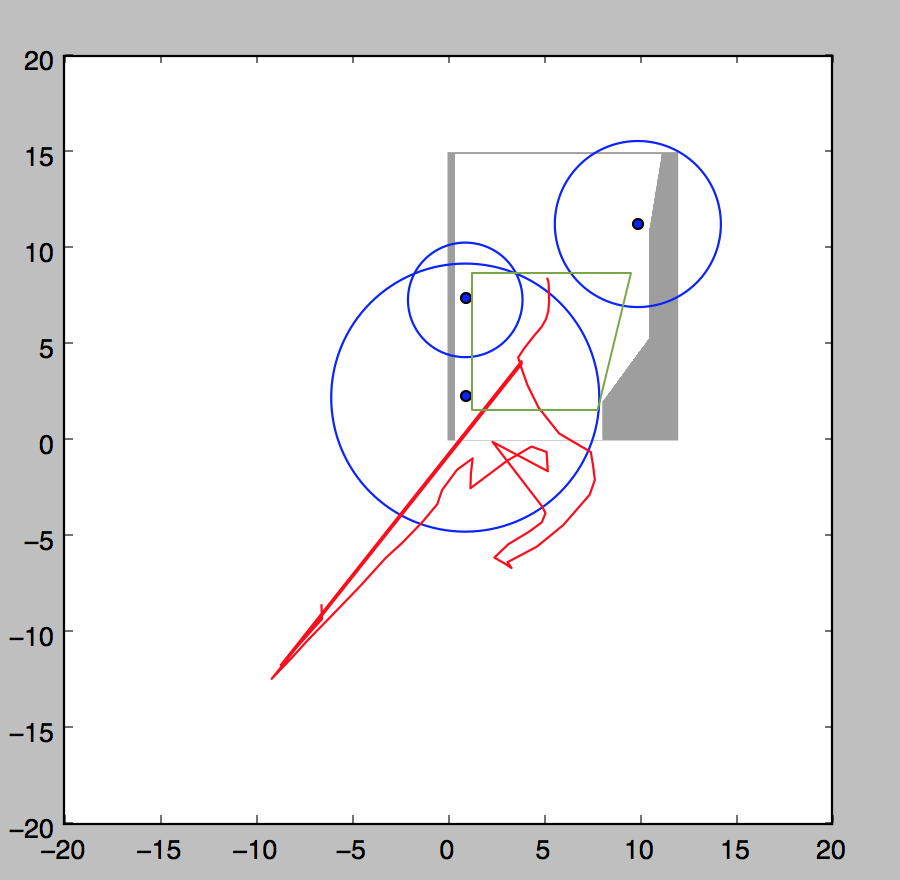
\includegraphics[width=0.45\textwidth]{figures/multilat_3}
  \label{fig:beacon_eval_multilat_3}
}
\subfloat[]{
  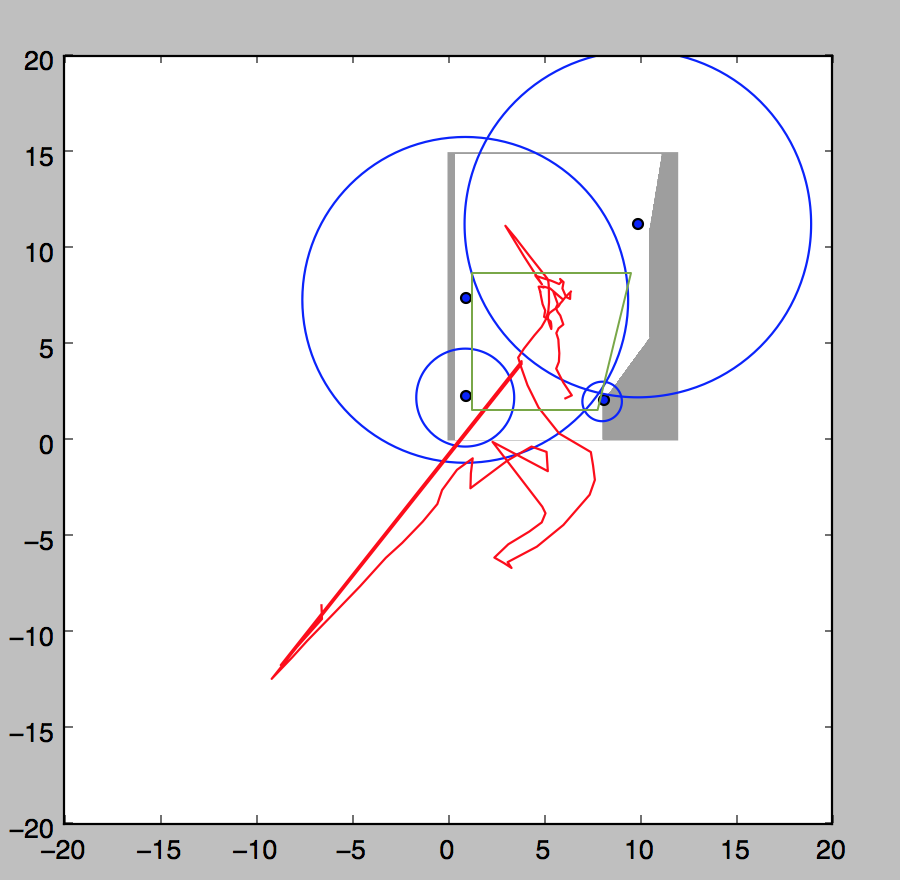
\includegraphics[width=0.45\textwidth]{figures/multilat_4}
}

  \caption{Screenshots of indoor self-localization experiment using multilateration.}
  \label{fig:beacon_eval_multilat}
\end{figure}

We repeated the experiment with the same data, but just used the beacon's signals where \texttt{accuracy} is $< 5~m$. Signals with larger estimated distances where ignored. Figure~\ref{fig:beacon_eval_multilat_less5m} shows the result. The estimated path actually is inside of the lecture hall. Its not possible to determine that the user walked on the green path, but ignoring values less than 5~m seem to improve the location estimation.

\begin{figure}
	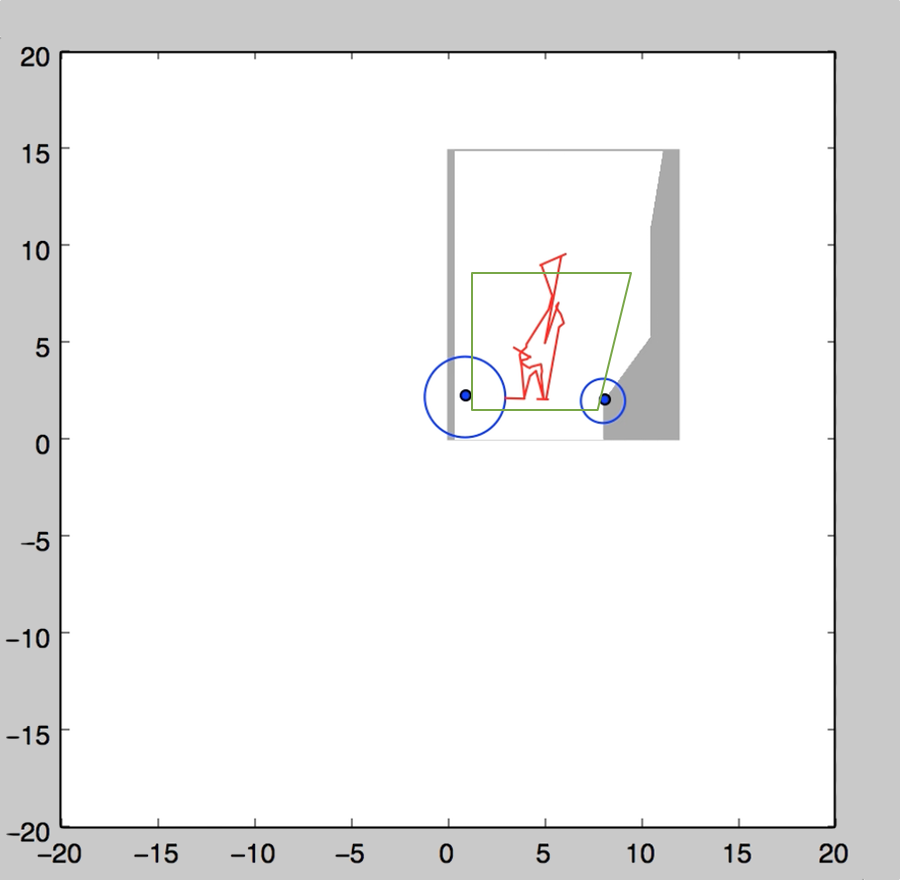
\includegraphics[width=0.45\textwidth]{figures/multilat_less5m}
	\caption{Screenshots of indoor self-localization experiment using multilateration, by using just signals where $\texttt{accuracy} < 5~m$.}
	\label{fig:beacon_eval_multilat_less5m}
\end{figure}

This experiment shows, that the beacons's signals must be heavily influenced, due to the very unreliable distance estimations. It also shows that pure multilateration, without filtering the data and without integrating additional data sources, is not sufficient enough for indoor self-localization.

\subsection{Summary}
The results show, that the distance estimation not just depend on the beacons calibration, it also depends on the buildings construction form, the phones relative attitude to the beacon, and the obstacles in between.

It also points out, that the \texttt{CLBeacon}'s \texttt{accuracy} resp.\ the estimated distance, comes very close to the actual distance up to 4--5~meters with \acs{LOS}. Larger distances cause a much higher spreading, and thus, a larger error. Physical material like humans and walls do cause attenuation, which results in a larger distance as it actually is. Besides that, the estimated distance is sometimes very small, relative to the actual distance.

To conclude, the estimated distances are very unreliable; thus, their plausibility should be proofed to filtered the measurements. But, due to the fact, that the validity cannot be proofed, without knowing the receivers exact position and the properties of all other influencing factors, which is a nontrivial problem in large buildings, the only thing that could be done, is to ignore beacons with an estimated distance larger than 5~meters. This solves of course not the problem with beacons, which appear to be closer as the actually are. From our point of view, no solution exists to solve this problem.